\documentclass[]{AVSSimReportMemo}
\usepackage{AVS}
\usepackage{colortbl}


\newcommand{\ModuleName}{celestialTwoBodyPoint}
\newcommand{\subject}{Guidance Module for Celestial Two Body Point}
\newcommand{\status}{Initial Version}
\newcommand{\preparer}{M. Cols}
\newcommand{\summary}{Generate the attitude reference to satisfy a primary attitude pointing constrain and the best as possible a secondary one.}


\begin{document}

\makeCover


%
% enter the revision documentation here
% to add more lines, copy the table entry and the \hline, and paste after the current entry.
%
\pagestyle{empty}
{\renewcommand{\arraystretch}{2}
\noindent
\begin{longtable}{|p{0.5in}|p{4.5in}|p{1.14in}|}
\hline
{\bfseries Rev}: & {\bfseries Change Description} & {\bfseries By} \\
\hline
Draft & initial copy & M. Cols \\
\hline

\end{longtable}
}

\newpage
\setcounter{page}{1}
\pagestyle{fancy}

\tableofcontents
~\\ \hrule ~\\

\newpage
\section{Module Input and Ouptut}
Table \ref{tab:inputNavTable} shows the input message from the navigation system.
\begin{table}[h!]
	\centering
	\caption{Input Navigation Message}
	\begin{tabular}{|l|l|l|p{3in}|}
		\hline
		\rowcolor{BrickRed}
		\textcolor{white}{Name} & \textcolor{white}{Type} & 
		\textcolor{white}{Length} & 
		\textcolor{white}{Description}  \\ \hline
		$\leftexp{N}{\bm{r}}_{B/N}$ & double [] & 3 & 
		Position vector of the spacecraft body-point with respect to the inertial frame in inertial frame components. \\ \hline
		$\leftexp{N}{\bm{v}}_{B/N}$ & double [] & 3 & 
		Velocity vector of the spacecraft body-point with respect to the inertial frame in inertial frame components \\ \hline
	\end{tabular}
	\label{tab:inputNavTable}
\end{table}


Table \ref{tab:inputCelTable} shows the input message from Spice about the main celestial body.
\begin{table}[h!]
	\centering
	\caption{Input Spice Primary Message}
	\begin{tabular}{|l|l|l|p{3in}|}
		\hline
		\rowcolor{BrickRed}
		\textcolor{white}{Name} & \textcolor{white}{Type} & 
		\textcolor{white}{Length} & 
		\textcolor{white}{Description}  \\ \hline
		$\bm{R}_P$  & double [] & 3 & 
		Position vector of the primary celestial object with respect to the inertial frame in inertial frame components . \\ \hline
		$\bm{v}_P$  & double [] & 3 & 
		Velocity vector of the primary celestial object with respect to the inertial frame in inertial frame components . \\ \hline
	\end{tabular}
	\label{tab:inputCelTable}
\end{table}


Table \ref{tab:inputSecTable} shows the input message from Spice about the secondary celestial body.
\begin{table}[h!]
	\centering
	\caption{Input Spice Secondary Message}
	\begin{tabular}{|l|l|l|p{3in}|}
		\hline
		\rowcolor{BrickRed}
		\textcolor{white}{Name} & \textcolor{white}{Type} & 
		\textcolor{white}{Length} & 
		\textcolor{white}{Description}  \\ \hline
		$\bm{R}_S$  & double [] & 3 & 
		Position vector of the secondary celestial object with respect to the inertial frame in inertial frame components . \\ \hline
		$\bm{v}_S$  & double [] & 3 & 
		Velocity vector of the secondary celestial object with respect to the inertial frame in inertial frame components . \\ \hline
	\end{tabular}
	\label{tab:inputSecTable}
\end{table}


Table \ref{tab:outputTable} shows the Attitude Reference output message of the module Celestial Two Body Point.
\begin{table}[h!]
	\centering
	\caption{Output Attitude Reference Message}
	\begin{tabular}{|l|l|l|p{3in}|}
		\hline
		\rowcolor{BrickRed}
		\textcolor{white}{Name} & \textcolor{white}{Type} & 
		\textcolor{white}{Length} & 
		\textcolor{white}{Description}  \\ \hline
		$\bm{\sigma}_{R/N}$ & double [] & 3 & 
		MRP attitude set of the reference frame with respect to the inertial. \\ \hline
		$\leftexp{N} {\bm{\omega}_{R/N}}$ & double [] & 3 & 
		Angular rate vector of the reference frame with respect to the inertial expressed in inertial frame components. \\ \hline
		$\leftexp{N} {\bm{\dot{\omega}}_{R/N}}$ & double [] & 3 & 
		Angular acceleration vector of the reference frame with respect to the inertial expressed in inertial frame components. \\ \hline
	\end{tabular}
	\label{tab:outputTable}
\end{table}
\newpage

\section{Reference Frame Definition}
This module computes a reference whose aim is to track the center of a primary target, e.g. pointing the communication antenna at the Earth, at the same time of trying to meet a secondary constraint as best as possible, e.g. a solar panel normal axis pointing the closest in the direction of the Sun.  It is important to note that two pointing conditions in a three-dimensional space compose an overdetermined problem. Thus, the main constraint is always priorized over the secondary one so the former can always be met.\\
Figure~\ref{fig:fig1} shows the case where Mars is the primary celestial body and the Sun is the secondary one. Note that the origin of the desired reference frame $\mathcal{R}$ is the position of the spacecraft.
\begin{figure}[htb]
	\centerline{
	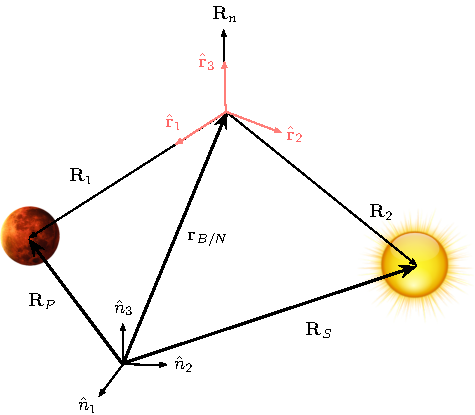
\includegraphics[]{Figures/fig1}
	}
	\caption{Illustration of the restricted two-body pointing reference frame $\mathcal{R}:\{ \hat{\bm r}_{1},\hat{\bm r}_{1}, \hat{\bm r}_{2} \}$ and the inertial frame $\mathcal{N}:\{ \hat{\bm n}_{1},\hat{\bm n}_{1}, \hat{\bm n}_{2} \}$.}
	\label{fig:fig1}
\end{figure}

Assuming knowledge of the position of the spacecraft $\bm{r}_{B/N}$ and the involved celestial bodies, $\bm{R}_{P1}$ and  $\bm{R}_{P2}$ (all of them relative to the inertial frame $\mathcal{N}$ and expressed in inertial frame components), the relative position of the celestial bodies with respect to the spacecraft is obtained by simple subtraction:
\begin{subequations}
	\begin{align}
		 \bm{R}_{P1} =\bm{R}_{P} - \bm{r}_{B/N} \\
		 \bm{R}_{P2} =\bm{R}_{S} - \bm{r}_{B/N} 
	\end{align}
\end{subequations}

In analogy, the inertial derivatives of these position vectors are obtained:
\begin{subequations}
	\begin{align}
		 \bm{v}_{P1} &=\bm{v}_{P} - \bm{v}_{B/N} \\
		 \bm{v}_{P2} &=\bm{v}_{S} - \bm{v}_{B/N} \\
		 \bm{a}_{P1} &=\bm{a}_{P} - \bm{a}_{B/N} \\
		 \bm{a}_{P2} &=\bm{a}_{S} - \bm{a}_{B/N} 
	\end{align}
\end{subequations}

The normal vector $\bm{R}_{n}$ of the plane defined by $\bm{R}_{P1}$ and $\bm{R}_{P2}$ is computed through:
\begin{equation}
	\bm R_{n} =\bm{R}_{P1} \times \bm{R}_{P2}
\end{equation}
The inertial time derivative of $\bm{R}_n$ is found using the chain differentiation rule:
\begin{equation}
	\bm {v}_{n} = \bm{v}_{P1} \times \bm{R}_{P2} + \bm{R}_{P1} \times \bm{v}_{P2} 
\end{equation}
And the second time derivative:
\begin{equation}
	\bm {a}_{n} = \bm{a}_{P1} \times \bm{R}_{P2} + \bm{R}_{P1} \times \bm{a}_{P2}  + 2 \bm{v}_{P1} \times \bm{v}_{P2} 
\end{equation}
\subsection{ Special Case: No Secondary Constraint Applicable}
If there is no incoming message with a secondary celestial body pointing condition or if the constrain is not valid, an artificial three-dimensional frame is defined instead. Note that a single condition pointing leaves one degree of freedom, hence standing for an underdetermined attitude problem. A secondary constrain is considered to be invalid if the angle between $\bm{R}_{P1}$ and $\bm{R}_{P2}$ is, in absolute value, minor than a set threshold. This could be the case where the primary and secondary celestial bodies are aligned as seen by the spacecraft. In such situation, the primary pointing axis would already satisfy both the primary and the secondary constraints.

Since the main algorithm of this module, which is developed in the following sections, assumes two conditions, the second one is arbitrarily set as following:
\begin{equation}
		 \bm{R}_{P2} = \bm{R}_{P1} \times \bm{v}_{P1} \equiv  \bm{h}_{P1}
\end{equation}
By setting the secondary constrain to have the direction of the angular momentum vector $ \bm{h}_{P1}$, it is assured that it will always be valid ($\bm{R}_{P1}$ and $\bm{R}_{P2}$ are now perpendicular).
The first and second time derivatives are steadily computed:
\begin{equation}
	\bm{v}_{P2} =  \bm{R}_{P1} \times \bm{a}_{P1} 
\end{equation}
\begin{equation}
	\bm{a}_{P2} =  \bm{v}_{P1} \times \bm{a}_{P1} 
\end{equation}
\section{Reference Frame Definition}
As illustrated in Figure~\ref{fig:fig1}, the base vectors of the desired reference frame $\mathcal{R}$  are defined as following:
\begin{subequations}
	\begin{align}
		\hat{\bm r}_{1} &= \frac{{\bm R}_{P1}} {|{\bm R}_{P1}|} \\
		\hat{\bm r}_{3} &= \frac{{\bm R}_{n}}{|{\bm R}_{n}|} \\
		\hat{\bm r}_{2} &=  \hat{\bm r}_{3} \times \hat{\bm r}_{1} 
	\end{align}
\end{subequations}
Since the position vectors are given in terms of inertial $\mathcal{N}$-frame components, the DCM from the inertial frame $\mathcal{N}$ to the desired reference frame $\mathcal{R}$ is:
\begin{equation}
	[RN] = \begin{bmatrix}
		\leftexp{N}{ \hat{\bm r}_{1}^{T} } \\
		\leftexp{N}{ \hat{\bm r}_{2}^{T} }  \\
		\leftexp{N}{ \hat{\bm r}_{3}^{T} }  
	\end{bmatrix}
\end{equation}
\section{Base Vectors Time Derivatives}
The first and second time derivatives of the base vectors that compound the reference frame $\mathcal{R}$ are needed in the following sections to compute the reference angular velocity and acceleration. Several lines of algebra lead to the following sets:
\begin{subequations}
	\begin{align}
		\dot{\hat{\bm{r}}}_1 &= ([I_{3\times3}] - {\hat{\bm{r}}_1}{\hat{\bm{r}}_1}^T)  \frac{{\bm R}_{P1}} {|{\bm R}_{P1}|} \\
		\dot{\hat{\bm{r}}}_3 &= ([I_{3\times3}] - \hat{\bm{r}}_3 \hat{\bm{r}}_3^T)  \frac{{\bm R}_{n}} {|{\bm R}_{n}|} \\
		\dot{\hat{\bm{r}}}_2 &= \dot{\hat{\bm{r}}}_3 \times \bm{r}_1 +  \bm{r}_n  \times \dot{\hat{\bm{r}}}_3 
	\end{align}
\end{subequations}

\begin{subequations}
	\begin{align}
		\ddot{\hat{\bm{r}}}_1 &= \frac{1}{|{\bm R}_{P1}|}
		(
		([I_{3\times3}] - {\hat{\bm{r}}_1}{\hat{\bm{r}}_1}^T)  \bm{a}_{P1} - 
		2\dot{\hat{\bm{r}}}_1 (\hat{\bm{r}}_1 \cdot \bm{v}_{P1}) - 
		\hat{\bm{r}}_1 (\dot{\hat{\bm{r}}}_1 \cdot \bm{v}_{P1}) 
		) \\
		\ddot{\hat{\bm{r}}}_3 &= \frac{1}{|{\bm R}_{n}|}
		(
		([I_{3\times3}] - {\hat{\bm{r}}_3}{\hat{\bm{r}}_3}^T)  \bm{a}_{n} - 
		2\dot{\hat{\bm{r}}}_3 (\hat{\bm{r}}_3 \cdot \bm{v}_{n}) - 
		\hat{\bm{r}}_3 (\dot{\hat{\bm{r}}}_3 \cdot \bm{v}_{n}) 
		) \\
		\ddot{\hat{\bm{r}}}_2 &= \ddot{\hat{\bm{r}}}_3 \times \bm{r}_1 +  \bm{r}_n  \times \ddot{\hat{\bm{r}}}_3 + 2\dot{\hat{\bm{r}}}_3 \cdot \dot{\hat{\bm{r}}}_1
	\end{align}
\end{subequations}

\section{Angular Velocity and Acceleration Descriptions}
Developing some more mathematics, the following elegant expressions of $\bm\omega_{R/N}$ and $\dot{\bm\omega}_{R/N}$ are found:
\begin{subequations}
	\begin{align}
		\bm\omega_{R/N} \cdot \hat{\bm r}_{1}  = \hat{\bm r}_{3} \cdot \dot{\hat{\bm r}}_{2}  \\
		\bm\omega_{R/N} \cdot \hat{\bm r}_{2} = \hat{\bm r}_{1} \cdot \dot{\hat{\bm r}}_{3}\\
		\bm\omega_{R/N} \cdot \hat{\bm r}_{3} = \hat{\bm r}_{2} \cdot \dot{\hat{\bm r}}_{1}
	\end{align}
\end{subequations}
\begin{subequations}
	\begin{align}
		\dot{\bm\omega}_{R/N} \cdot \hat{\bm r}_{1} &=  
		\dot{\hat{\bm r}}_{3} \cdot \dot{\hat{\bm r}}_{2} + \hat{\bm r}_{3} \cdot \ddot{\hat{\bm r}}_{2} -  \bm\omega_{R/N} \cdot \dot{\hat{\bm r}}_{1}
		\\
		\dot{\bm\omega}_{R/N} \cdot \hat{\bm r}_{2} &= 
		 \dot{\hat{\bm r}}_{1} \cdot \dot{\hat{\bm r}}_{3} + \hat{\bm r}_{1} \cdot \ddot{\hat{\bm r}}_{3} -  \bm\omega_{R/N} \cdot \dot{\hat{\bm r}}_{2}	
		\\
		\dot{\bm\omega}_{R/N} \cdot \hat{\bm r}_{3} &=  
		\dot{\hat{\bm r}}_{2} \cdot \dot{\hat{\bm r}}_{1} + \hat{\bm r}_{2} \cdot \ddot{\hat{\bm r}}_{1} -  \bm\omega_{R/N} \cdot \dot{\hat{\bm r}}_{3}
	\end{align}
\end{subequations}
Note that $\bm\omega_{R/N} \cdot \hat{\bm r}_{1}$ is the first component of the angular velocity of the reference with respect to the inertial expressed in reference frame components. Hence,
\begin{equation}
	\bm\omega_{R/N}= \leftexp{R}{
		\begin{bmatrix}
			\bm\omega_{R/N} \cdot \hat{\bm r}_{1} \\
			\bm\omega_{R/N} \cdot \hat{\bm r}_{2}  \\
			\bm\omega_{R/N} \cdot \hat{\bm r}_{3} 
		\end{bmatrix}
	}
\end{equation}
Similarly for the angular acceleration:
\begin{equation}
	\bm{\dot\omega}_{R/N} = \leftexp{R}{
		\begin{bmatrix}
			\bm{\dot\omega}_{R/N} \cdot \hat{\bm r}_{1} \\
			\bm{\dot\omega}_{R/N} \cdot \hat{\bm r}_{2}  \\
			\bm{\dot\omega}_{R/N} \cdot \hat{\bm r}_{3} 
		\end{bmatrix}
	}
\end{equation}
Eventually, in inertial frame components:
\begin{subequations}
	\begin{align}
		\leftexp{N} {\bm\omega_{R/N}} &= [RN] \textrm{ } \leftexp{R} {\bm\omega_{R/N}} 
		\\
		\leftexp{N} {\bm{\dot\omega}_{R/N}} &= [RN]  \textrm{ } \leftexp{R} {\bm{\dot\omega}_{R/N}}
	\end{align}
\end{subequations}

\bibliographystyle{unsrt}
\bibliography{references}

\end{document}
